\chapter{M\'odulo de Dashboard}

\section{Descripci\'on General}

El dashboard proporciona una vista general del estado de la cl\'{\i}nica
con m\'etricas en tiempo real obtenidas directamente de la base de datos.
Utiliza \texttt{cache()} de React para optimizar el renderizado del lado
del servidor.

\section{Consulta de M\'etricas}

\begin{lstlisting}[style=typescript, caption=getDashboardMetrics - Consultas paralelas]
export const getDashboardMetrics = cache(
  async function getDashboardMetrics(): Promise<DashboardMetrics> {
    const clinicId = await getCurrentClinicId();
    const today = new Date().toISOString().slice(0, 10);
    const monthStart = new Date();
    monthStart.setDate(1);
    const monthStartStr = monthStart.toISOString().slice(0, 10);

    // 8 consultas en paralelo
    const [apptsAgg, clientsCount, patientsCount,
           invoicesAgg, upcoming, recentClients,
           recentPatients, recentInvoices] =
      await Promise.all([

        // 1. Citas de hoy agrupadas por estado
        db.select({
          status: schema.appointments.status,
          count: sql<number>`count(*)`,
        }).from(schema.appointments)
          .where(and(clinicFilter,
                eq(schema.appointments.date, today)))
          .groupBy(schema.appointments.status),

        // 2-3. Total de clientes y pacientes
        db.select({ count: sql<number>`count(*)` })
          .from(schema.clients).where(clinicFilterClients),
        db.select({ count: sql<number>`count(*)` })
          .from(schema.patients).where(clinicFilterPatients),

        // 4. Ingresos de hoy y del mes
        db.select({
          today: sql<number>`coalesce(sum(total) filter
            (where created_at >= ${today}::timestamp), 0)`,
          month: sql<number>`coalesce(sum(total) filter
            (where created_at >= ${monthStartStr}::timestamp), 0)`,
        }).from(schema.invoices)
          .where(and(clinicFilterInvoices,
                eq(schema.invoices.status, 'paid'))),

        // 5. Proximas 5 citas
        db.select({...})
          .from(schema.appointments)
          .innerJoin(...)
          .where(and(clinicFilter,
                gte(schema.appointments.date, today)))
          .orderBy(schema.appointments.date,
                   schema.appointments.startTime)
          .limit(5),

        // 6-8. Actividad reciente (5 de cada tipo)
        db.select({...}).from(schema.clients)
          .where(clinicFilterClients)
          .orderBy(desc(schema.clients.createdAt)).limit(5),
        db.select({...}).from(schema.patients)
          .where(clinicFilterPatients)
          .orderBy(desc(schema.patients.createdAt)).limit(5),
        db.select({...}).from(schema.invoices)
          .where(clinicFilterInvoices)
          .orderBy(desc(schema.invoices.createdAt)).limit(5),
      ]);
    // ... procesamiento de resultados ...
  }
);
\end{lstlisting}

\section{Componentes del Dashboard}

\subsection{Tarjetas de Resumen (4)}

\begin{itemize}[leftmargin=*]
    \item \textbf{Citas Hoy:} Conteo total y desglose de pendientes.
          Icono: Calendar, enlace a /appointments.
    \item \textbf{Clientes:} Total registrados. Icono: Users,
          enlace a /clients.
    \item \textbf{Pacientes:} Total activos. Icono: PawPrint,
          enlace a /patients.
    \item \textbf{Ingresos:} Total hoy y del mes. Icono: DollarSign,
          enlace a /invoices.
\end{itemize}

Cada tarjeta tiene un gradiente de fondo, animaci\'on hover (scale + y-offset)
y transici\'on de entrada con Framer Motion.

\subsection{Panel de Pr\'oximas Citas}

\begin{itemize}[leftmargin=*]
    \item Muestra hasta 5 citas pr\'oximas.
    \item Cada cita: hora, nombre del paciente (con icono de huella),
          due\~no, tipo y estado con color sem\'antico.
    \item Manejo de estado vac\'{\i}o con mensaje informativo.
\end{itemize}

\subsection{Panel de Actividad Reciente}

\begin{itemize}[leftmargin=*]
    \item Combina y ordena los \'ultimos 5 eventos de clientes, pacientes
          y facturas.
    \item M\'aximo 10 eventos, ordenados por fecha descendente.
    \item Puntos de colores seg\'un tipo (azul=cliente, verde=paciente,
          \'ambar=factura).
    \item Animaci\'on de pulso en los puntos indicadores.
\end{itemize}

\section{P\'agina del Dashboard}

La p\'agina (\texttt{/(dashboard)/page.tsx}) es un Server Component que:

\begin{enumerate}
    \item Verifica la sesi\'on del usuario.
    \item Obtiene las m\'etricas del dashboard.
    \item Pasa los datos al \texttt{AnimatedDashboardClient} (client component).
\end{enumerate}

\section{Optimizaci\'on}

\begin{itemize}[leftmargin=*]
    \item \textbf{cache():} La funci\'on \texttt{getDashboardMetrics} est\'a
          envuelta en \texttt{cache()} de React para deduplicar llamadas.
    \item \textbf{Promise.all:} Las 8 consultas SQL se ejecutan en paralelo.
    \item \textbf{Server Component:} El renderizado inicial ocurre en el
          servidor, minimizando JavaScript del lado del cliente.
\end{itemize}

\begin{figure}[H]
    \centering
    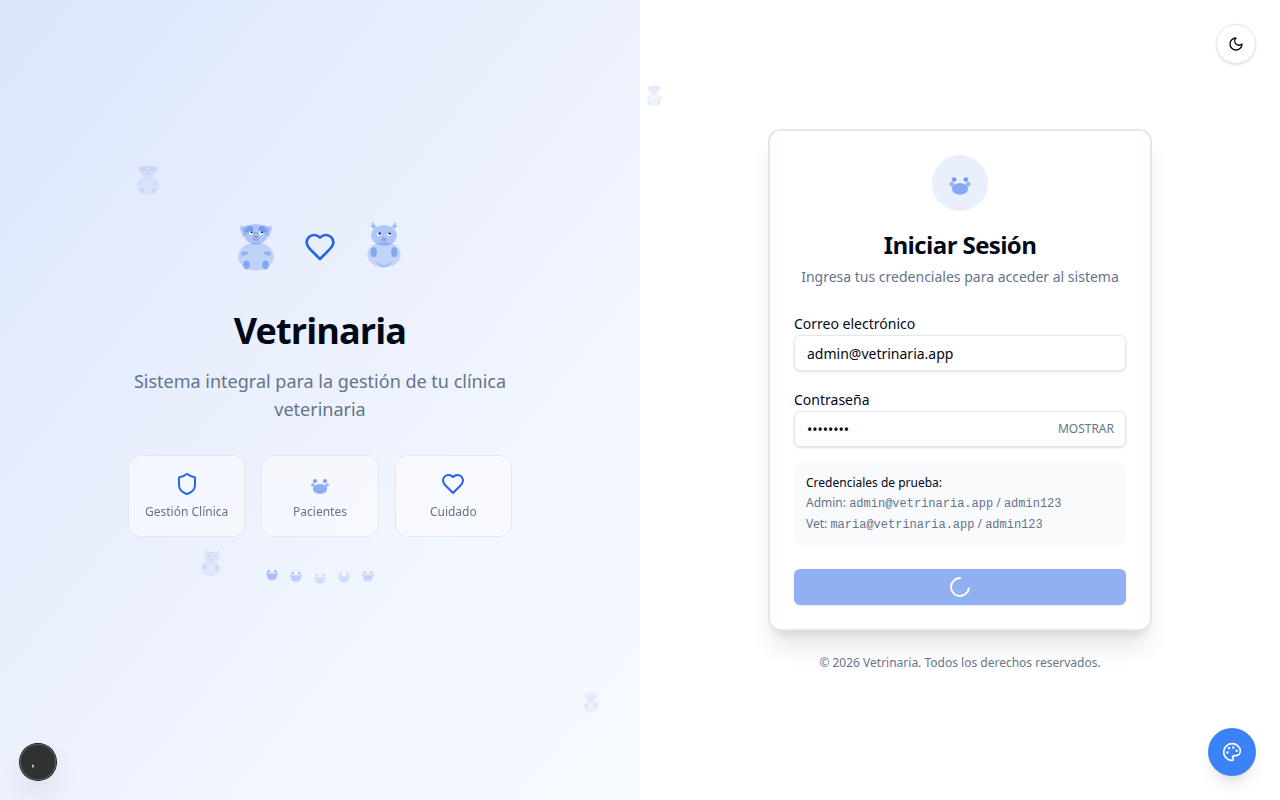
\includegraphics[width=\textwidth]{img/vet-dashboard.png}
    \caption{Dashboard principal con metricas en tiempo real}
    \label{fig:dashboard}
\end{figure}
